\section{Quantum Bits}

Classical computation is built upon \textit{bits}. In the world of Quantum computation and quantum information, we have an analogous concept known as a \textit{quantum bit}, or \textit{qubit}.

\begin{definition}[Classical Bit]
	A \textit{classical bit} is a unit of information that takes on one of two states, commonly denoted 0 or 1. The term bit is a portmanteau of the term binary digit.
\end{definition}

\begin{definition}[Quantum Bit]
	A quantum bit, also known as a qubit has a state. Two possible states for a qubit are $ \ket{0} $ and $ \ket{1}. $ The notation $ ``\ket{  \ }" $ is known as \textit{Dirac notation} named after Paul Dirac.
\end{definition}

The main difference between bits and qubits is that a qubit can take on a state other than $ \ket{0} $ or $ \ket{1}. $ A qubit can take the form that is a linear combination of these two states, this is referred to as a superposition.

An example of a superposition is the following
\begin{equation}\label{superpos_eq}
\ket{\psi} = \alpha \ket{0} + \beta \ket{1},
\end{equation}
where $ \alpha, \beta \in \mathbb{C}. $

We can consider the state of a qubit as a vector in $ \mathbb{C}^2. $ The states $ \ket{0} $ and $ \ket{1} $ are known as computation basis states and form an orthogonal basis for this vector space.

While a bit's state can be determined by examination, the same is not true for a qubit. That is, one cannot determine the values $ \alpha $ and $ \beta. $ When we measure a qubit we either get the result 0, with probability $ \left| \alpha \right|^2, $ or the result 1, with probability $ \left| \beta \right|^2. $ Since the total probability must sum to 1, we have that $ \left| \alpha \right|^2 + \left| \beta \right|^2 = 1. $ Returning to the vector space interpretation, we have that the qubit's state is a unit vector in $ \mathbb{C}^2. $

\begin{example}
	A qubit can have the following state, \[ \frac{1}{\sqrt{2}}\ket{0} + \frac{1}{\sqrt{2}}\ket{1}, \] when measured the state gives the result 0 fifty percent of the time, as well as the result 1 fifty percent of the time. This state is commonly denoted $ \ket{+}. $
\end{example}

We can think about qubits using a different geometric interpretation by rewriting Equation (\ref{superpos_eq}) as
\begin{equation}
\ket{\psi} = e^{i \gamma} \left[ \cos\left(\frac{\theta}{2}\right)\ket{0} + e^{i \phi}\sin\left(\frac{\theta}{2}\right)\ket{1} \right],
\end{equation}
where $ \theta, \phi, \gamma \in \mathbb{R}. $ We will later see that we can ignore the factor of $ e^{i\gamma}, $ because it has no observable effects. We can now write
\begin{equation}
\ket{\psi} = \cos\left(\frac{\theta}{2}\right)\ket{0} + e^{i \phi}\sin\left(\frac{\theta}{2}\right)\ket{1},
\end{equation}

where the numbers $ \theta $ and $ \phi $ define a point on the three-dimensional unit sphere. We will refer to this as the \textit{Bloch sphere.}

\begin{figure}[H]
	\centering
	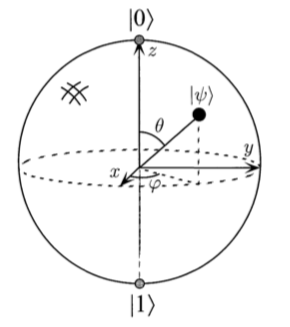
\includegraphics[scale = 0.5]{bloch_sphere}
	\caption{Bloch Sphere REFERENCE}
\end{figure}

\subsection{Multiple Qubits}

With two classical bits, there are four possible states: 00, 01, 10, and 11. Similarly, qubits have the four corresponding computation basis states: $ \ket{00}, \ket{01}, \ket{10}, $ and $ \ket{11}. $

A pair of qubits can also exist in superposition. This can be represented as the following \[ \ket{\phi} = \alpha_{00}\ket{00} + \alpha_{01}\ket{01} + \alpha_{10}\ket{10} + \alpha_{11}\ket{11}. \] Where each $ \alpha_{ij} $ is a complex coefficient, known as the \textit{amplitude}. The measurement result for each of the four states occurs with probability $ \left| \alpha_{ij} \right|^2 $